  \section{Bibtex}
\label{sec:Bibtex}
	

\begin{center}
	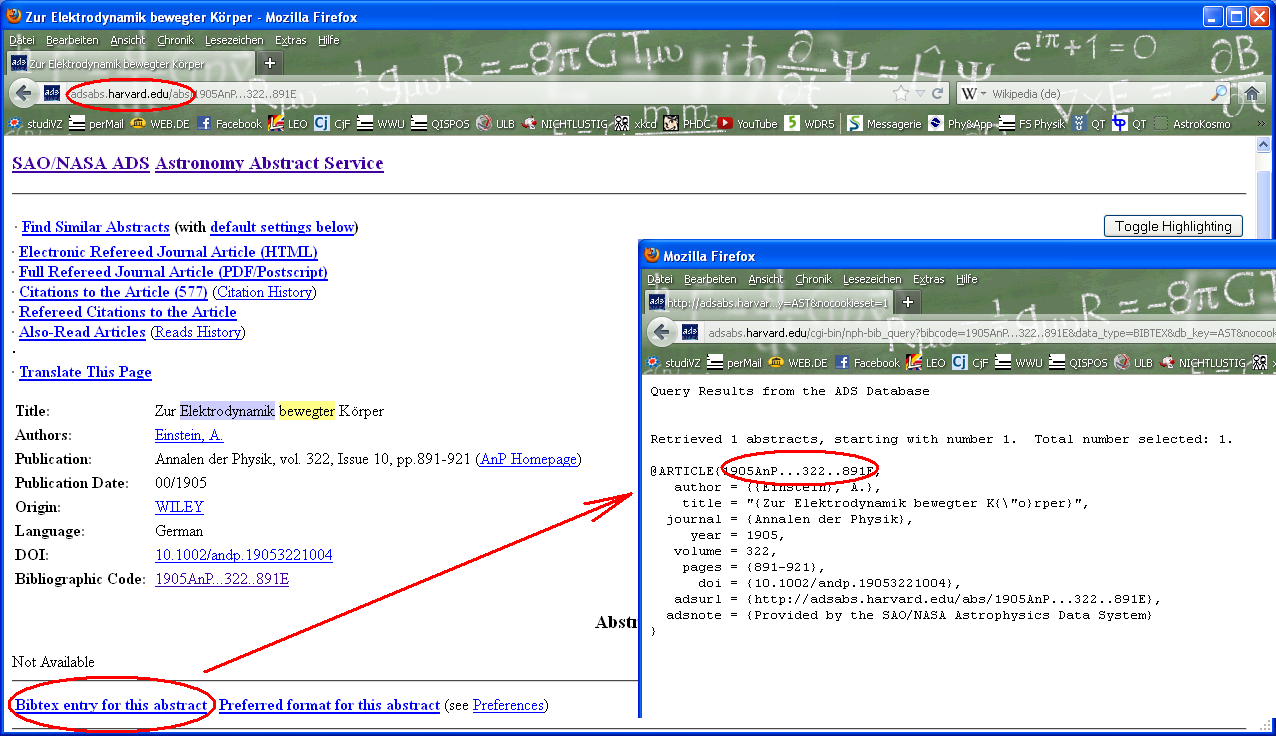
\includegraphics[width=1.00\textwidth]{adsabs}
\end{center}

Hier ist ganz viel Text und ein Zitat: (\verb+\cite{1905Einstein}+) \cite{1905Einstein}.

Das Programm $\verb+bibtex+$ erm�glicht es, Literaturangaben aus einer Datenbank (Textdatei mit Endung: .bib) zu holen.
Es werden im Literaturverzeichnis nur die Werke aufgef�hrt, die auch wirklich im Text zitiert werden.
Das Literarturverzeichnis selbst fordert man an mit:
\begin{verbatim}
\bibliographystyle{amsplain}
\bibliography{lit}
\end{verbatim}
Die Kompilierungsreihenfolge ist in diesem Fall:
\begin{itemize}

	\item
	pdflatex dateiname
	
	\item
	bibtex dateiname
	
	\item
	pdflatex dateiname

	\item
	pdflatex dateiname
	
\end{itemize}

\bibliographystyle{amsplain}
\bibliography{lit}

